\documentclass[12pt]{article}

\linespread{1.6}

\usepackage{amsmath}
\usepackage{amsfonts}
\usepackage{amssymb}
\usepackage{amsthm}

\newtheorem{lemma}{Lemma}
\newtheorem*{lemma*}{Lemma}
\newtheorem{theorem}{Theorem}
\newtheorem*{theorem*}{Theorem}

%\addtolength{\topmargin}{-.875in}
%\addtolength{\textheight}{1.75in}
\usepackage{graphicx}

\usepackage{caption} 
\captionsetup[table]{skip=12pt}
\captionsetup[table]{labelfont=bf}

\captionsetup[figure]{labelfont=bf}

\title{Capstone Project 2 Report\\ Training a Neural Net to Play Chess}
\author{Brian Lubeck}

\begin{document}
	\maketitle

\section{Introduction}

\subsection{Some Game Theory Background}
%Basic Definitions
%Zermelo's theorem and Kuhn's theorem
%Minimax Algorithm

Chess is the classic example of a (finite) two-person, zero-sum game. A two-person, zero-sum game is a game such that for any end to the game, if the payoff to player 1 is $p$, then payoff to player 2 is $-p$. In other words, the sum of the payoffs is always zero. In addition, chess is also an example of a game of perfect information. This means that a player, when it's his turn, knows exactly which node he is at in the game tree, how he arrived at the node and every possible future node for any sequence of moves. The main theoretical result regarding games of perfect information is a theorem proved by Kuhn. \cite{hart}

\begin{theorem*}[Kuhn (1953)] Every (finite) n-person game of perfect information has an equilibrium point in pure strategies.
\end{theorem*}

An equilibrium point is a set of pure strategies such that a player cannot increase his payoff by changing his pure strategy assuming the other players do not change their pure strategies. The proof is by induction where the player whose turn it is chooses the subtree that has highest equilibrium payout for the player. In the case of Chess, if we assign $1$ for a win, $0$ for a draw and $-1$ for a loss, then this theorem implies that either White can force a win, Black can force a win or both players can force a draw. At this point in time, it is still unknown which of the three outcomes is the correct one.\footnote{https://en.wikipedia.org/wiki/Solving\_chess}

The inductive proof of the theorem gives rise to a recursive method to find, in theory, the optimal pure strategy in any n-person game of perfect information. For two-person, zero-sum games, this recursive method is known as the minimax algorithm. To find the optimal pure strategy for each player, we grow the game tree all the way to its terminal nodes, where each terminal node has a payoff of 1 for a win, 0 for a draw or -1 for a loss for the first player. Retracing the game tree from the terminal nodes to the root node, we select at each node the move that maximizes the payoff if it is the first player's turn or the move that minimizes the payoff if it is the second player's turn. For games with small game trees, such as Tic-Tac-Toe, we can use a computer to go through the entire game tree to find the optimal move. For games with large game trees, we can also use a computer to go through the entire game tree since the game tree is finite; however, the time required to do so may make searching the entire game tree practically impossible. In the case of chess, Claude Shannon estimated that the game tree has at \textit{least} $10^{120}$ paths from the root node to a terminal node. \cite{shannon} Deep Blue, the first computer ever to beat the world chess champion in 1996 and the computer that marked the superiority of brute-force computational speed over human thinking at chess, could examine $200$ million nodes per second.\footnote{http://www.talkchess.com/forum/viewtopic.php?t=48387} Another program, written to run on an Nvidia GTX 780 GPU, could examine $20$ billion nodes per second.\footnote{http://www.talkchess.com/forum/viewtopic.php?t=48387} Even at $20$ billion nodes per second, it would take a computer at least $10^{90}$ years to calculate the correct first move. Thus, since this is impractical, an alternative method must be employed in order to find a good move. The basic algorithm to overcome this obstacle and the one employed by the majority of modern chess engines is to use an abbreviated minimax search along with an evaluation function. Thus, a good search algorithm and a good evaluation function are essential features of any decent chess program since it is infeasible to search the entire game tree.\footnote{ See https://chessprogramming.wikispaces.com/Search and ./Evaluation for a comprehensive discussion of search techniques and evaluation criteria used by chess engines.} We first briefly discuss the main search techniques used by most chess engines, and then we briefly discuss the main evaluation criteria used by most chess engines.

\subsection{Basic Elements of a Chess Engine}
%Board Representation - Bitboards
%Search - Minimax Algorithm
%		Alpha-Beta Pruning
%		Transposition Table
%		Quiesecence Search ? keep deepening until no higher piece threatened by lower piece? Example of combination between search and eval
%		Parallel code - DTS
%		PSV iterative deepening
% 		Null move
%		Horizon Effect
% Evaluation
%	main ideas - material, tempo, mobility, endgame vs middlegame
%	all this info contained in board - let nn pick out important features instead of
For most chess engines, the minimax algorithm is the foundational basis for the search algorithm. In its most basic implementation, the game tree is grown depth-first to a certain depth, and at each terminal node an evaluation function is called that estimates the relative value of the terminal node, i.e. the chances of winning or losing. Beyond the basic minimax algorithm, the main techniques used to improve the search algorithm are:
\begin{enumerate}
	\item Alpha-Beta Pruning
	\item Transposition Table
	\item Iterative Deepening
	\item Aspiration Windows
\end{enumerate}

Alpha-Beta pruning is a refinement to the basic minimax algorithm that on averages decreases the number of nodes needed to be searched on average to find the optimal move. For a fixed a amount of time, this allows the game tree to be grown on average to a greater depth. As the game tree is searched two values are saved, alpha and beta. Alpha is the best value that the maximizer can currently guarantee at that depth or below and beta is the best value that the minimizer can currently guarantee at that depth or below. While searching over a subtree, if alpha becomes greater than or equal to beta, then searching that subtree can be stopped.

In chess a transposition is a sequence of moves that results in a board position that is reachable by a different sequence of moves. Transpositions in chess are common. As a result, a table called a transposition table is used that stores information about previously searched board positions. A transposition table is typically implemented as a hash table.

Frequently chess games are played under a time-control. For example, for standard tournaments, FIDE rules recommend 90 minutes for the first 40 moves followed by 30 minutes for the rest of the game and an addition of 30 seconds per move starting from move one. In contrast, for the FIDE World Blitz Championship, each player has 3 minutes plus 2 seconds per move to finish the game. Thus, a chess engine must have some strategy to manage the amount of time spent "thinking" about a move. Iterative deepening is a refinement to depth-first search algorithms. It first grows the game tree to a depth of one and evaluates the terminal nodes. It then repeatedly grows the game tree one level deeper and evaluates the new terminal nodes until time is up. It is the basic time management strategy used by chess engines that use depth-first searches.

In alpha-beta pruning, alpha and beta are initialized to negative and positive infinity, respectively. An aspiration window is the range specified by alpha and beta. Aspiration windows is a heuristic algorithm that tries to reduce the number of nodes to be searched using alpha-beta pruning. It works by taking the score of the game tree, usually the score from the latest depth in iterative deepening, and sets alpha and beta to be close to this score.\footnote{https://chessprogramming.wikispaces.com/Aspiration+Windows} Beyond these four main techniques, researchers, programmers and chess enthusiats have experimented with many ideas to improve a chess engine's search algorithm. One notable idea has been to parallelize the search algorithm by taking advantage of multi-core CPUs or GPUs, resulting in a significant speed up.

Having briefly described the main search techniques used by most chess engines, we now briefly discuss evaluation functions used by chess engines. Recall that an evaluation function is a function that determines the relative value of a board position based on features of the board position. An evaluation function can be light or heavy. A light evaluation function utilizes at most a few basic features of the position. Two common ones are material worth and piece-square tables. Each chess piece is given a base value. A common rule of thumb is that a pawn is worth 1, a knight or bishop is worth 3, a rook is worth 5 and a queen is worth 9. A chess piece's value can be different depending on the square on which it is located. For example, a white knight at c3 is usually worth more than a knight at b1 since it attacks the center square d5. Thus, a piece-square table can be used, one for each piece, that adds an incremental amount to the piece's base value based on the square it occupies. In contrast to a light evaluation function, a heavy evaluation function is one that incorporates many features of the board position. The more features used, the heavier the function. For example, players are taught that doubled pawns are bad but passed pawns are good, so a heavy evaluation function might subtract an amount for doubled pawns but add an amount for passed pawns to the base value.

\subsection{Neural Networks and Chess}
%neural net to evaluate board
% 	deep pink's formula based on assumption of optimal play, but chess in theory
%   should always be able to force a draw? data doesn't reflect draw
%   early attempts - hardwarde, gpus didn't exist?
%   master thesis critique
% Neural Networks
% human knowledge
%	computers have worked out all endgame positions with 7 or fewer pieces
%	exs - stockfish and gnu chess
%	neural network attemtps
%		deep pink
%		chess programming two people
%		master thesis
Regardless of its complexity, chess evaluation functions have traditionally been linear functions with features learned soley from human knowledge.\footnote{https://chessprogramming.wikispaces.com/Evaluation} In contrast, neural networks are a class of functions known for their ability to learn complex relationships, which are often too hard for humans to learn. Previous work into using neural networks and machine learning techniques to play chess has been conducted. Wiering, Patist and Mann \cite{wiering} used a reinforcement learning method called temporal differences and a database of 50,000 games to train seven different feed-forward neural networks to evaluate a board position. Their neural networks had one hidden layer with 80 nodes and an output layer with one node. A variety of different features about the position, such as material, piece mobility and piece connectivity, were used for the input layer. To test their neural networks, they modified an open source chess engine to use their neural networks. They then played a tournament among the neural network modified chess engines and the original, unmodified chess engine where each engine played 5 games as white and 5 games as black against the other engines. The search depth was limited to two half-moves for all engines. Their best neural network consisted of three different neural networks, one for the opening, middle-game and endgame and beat the original chess engine 7 out of 10 times. Erik Bern \cite{bern} used a neural network that consisted of an input layer with 768 nodes, three hidden layers each with 2,048 nodes and an output layer with one node. To train the neural network, he used 100 million games from the FICS games database\footnote{https://www.ficsgames.org/download.html} and a custom loss function derived from the assumptions that white and black always made optimal moves or near optimal moves and that any other move was always worse. Lastly, Matthew Lai \cite{lai} for his master's thesis trained a feed-forward neural network using a temporal difference method called TDLeaf($\lambda$) and a training set of 5 million randomly selected positions as initial positions for self-play. TDLeaf($\lambda$) is method that allows faster learning by exploiting the fact that the local gradient of minimax is simply the gradient of the evaluation function at the leaf node of the search. Using the trained neural network Lai was able to create a chess program with an ELO rating of 2400, which is considered International Master level.

\subsection{Analysis Goals}
%Goal
%	The strength of a chess program can be improved by using a neural network 
%	chess engine's main evaluation function
%Important Capabilities of Chess Engines
%Number of nodes/half moves generated per second
%Accurate board eval
%Potential trade off between the two
While the previous work has shown that a neural network can be used as the board evaluation function to create a strong chess program, it has not completely explored the incremental trade-off between search and evaluation. Given a fixed amount of time to find a move, the more time it takes to calculate an evaluation function, the less time there is to search different board positions. Thus, there is a trade-off between the complexity of an evaluation function and the exhaustiveness of a search. To investigate this trade-off and to understand the benefit of a neural network with regards to chess, we examined three hypotheses:
\begin{description}
	\item[Hypothesis 1] There exists a neural network such that it can consistently beat a traditional evaluation function given a fixed search depth.
	\item[Hypothesis 2] There exists a neural network such that it can consistently beat a traditional evaluation function given a fixed amount of time per move. In other words, a neural network needs less time per move than a traditional evaluation function to play at the same strength.
	\item[Hypothesis 3] A neural network's greatest value is to evaluate a "quiet" position rather than a tactical one.
\end{description} 

Computers analyze a position with the help of their
%chess knowledge. The more chess knowledge it has, the longer it takes for a single position
%to be evaluated. So the playing strength not only depends on the amount of knowledge,
%it also depends on the time it takes to evaluate a position, because less evaluation-time
%leads to deeper searches. It is a question of finding a balance between chess knowledge
%and search depth which is also called the search/knowledge trade-off [8]. Deep Blue for
%instance, relied mainly on a high search depth. Other programs focus more on chess
%knowledge and therefore have a relatively lower search depth.
Answers to these hypotheses will help show what the trade-off is between a sophisticated evaluation function that is presumably more accurate but constrains the search versus a simpler function that is presumably less accurate but does not constrain the search. In addition, this analysis will help show under what conditions a neural network is appropriate for chess and other games of perfect information and how a neural network should be used.

\section{Data and Methodology}
To evaluate these hypotheses, we needed two main ingredients - a neural network and a chess program to modify to use either a neural network or a traditional board evaluation function. For the neural network, we built and trained a feed-forward neural network using games from the Free Internet Chess Server (FICS) database\footnote{https://www.ficsgames.org/download.html} and for the chess program, we chose an open source chess engine written in C by Tom Kerrigan\cite{tscp} because the source code was relatively easy to understand and modify. We created a copy of the source code and modified it to use our neural network. We then conducted several experiments where each experiment consisted of the modified program and the original program playing twenty games - ten as white and ten as black - under different parameters. For each game, we recorded the outcome, the average number of board positions searched and the average time per move. Table \ref{t1} below list the parameters for the different experiments.

\begin{table}[h]
	\centering
	\caption{Experimental Parameters} \label{t1}
	\begin{tabular}{l  r r r r r r r}
		\multicolumn{1}{c}{Experiment} & \multicolumn{1}{c}{Parameter} &  \multicolumn{1}{c}{Values}\\ \hline
		1 & Search Depth & 2, 4, 6 Half-Moves \\
		2 & Time per Move & 1, 2, 5 Seconds \\
		3 & Position Type & Quiet vs. Tactical \\
		\hline
	\end{tabular}
\end{table}
% H1, H2, H3 Train neural network
% H1, H2, H3 Data - FICS databases, number of games, number of positions, distribution ratings, white/draw/black winning percentage, rating gap and winning, num og games, ave moves per game, 2006-2009 data
%H1, H2, H3 Modified open source chess engine TCSP so that an adequate number of nodes is searched, For depth = 1 to 8, played programs against each other 20 times - 10 times as white and black, Fixed time at 1 sec for original program, then modified time for neural network (record average number of nodes searched), 2nd version of code where neural network is only called to evaluate positional states.



%The programs can look very deep ahead nowadays, so they are quite good at calculating
%tactical lines. Winning material in chess usually occurs within a few moves and most chess
%programs have a search depth of at least 8 ply. Deeper search can occur for instance, when
%a tactical line is examined or a king is in check after normal search or if there are only
%a few pieces on the board. Humans are able to recognize patterns in positions and have
%therefore important information on what a position is about. Expert players are quite
%good at grouping pieces together into chunks of information, as was pointed out in the
%psychological studies by de Groot [12]. 

%Show relevant sections of modified code

\subsection{Overview of the Data}
To train the neural network, we used chess games from 2006 to 2009 played on FICS's website between players with a combined average rating greater than 2000. We chose to use master level games because games between low rated players often have many blunders. As a result, we had more confidence that master level games were closer to the true relationship between a board position and game outcome. For example, if a player is up a rook, then the player should be able to win the majority of the time. We had more confidence that a master level player would convert this material advantage into a win than a low rated player. On the other hand, since master level players are less likely to blunder, the chances of such a material advantage occurring during a game are slim. This indicates a potential gap in the training data of example board positions that are clearly bad. Lastly, we note that although master level players are good by human standards, they are far from perfect players. In our database of chess games, white won 47.51\% of the games, lost 43.86\% of the games and drew 8.63\% of the games. From Kuhn's theorem, it follows that if they were perfect players then every game should have been a white win, loss or draw 100\% of the time. Table \ref{t2} below lists some statistics about our chess database, and Figure 1 shows how evenly matched the games were.  %1. Didn't use games between low rated players because low rated players could have %relationships that are bad to learn
%for example, a if white is up a rook, this position should lead to a win 99%+ of the %time, but with bad players this position might lead to a win only 50% of the time %because bad players blunder a lot
%2. further training = neural net plays against itself and one of the player's make a %mistake occassionally
%3. skill level game = sum of 2 players and use this as a weight, rating diff between %players

\begin{table}[h]
	\centering
	\caption{Chess Database} \label{t2}
	\begin{tabular}{l r r r r r r r}
		\multicolumn{1}{c}{Description} & \multicolumn{1}{c}{Value} \\ \hline
		Years & 2006 to 2009 \\
		Number of Games & 1,158,000 \\
		Number of Board Positions & 96,239,309 \\
		Average Number of Full Moves per Game & 41.55 \\
		White Winning Percentage & 47.51\% \\
		Black Winning Percentage & 43.86\% \\
		Draw Percentage & 8.63 \% \\
		\hline
	\end{tabular}
\end{table}

\begin{figure}[h!]
	\centering
	\caption{Histogram of Rating Differences}
	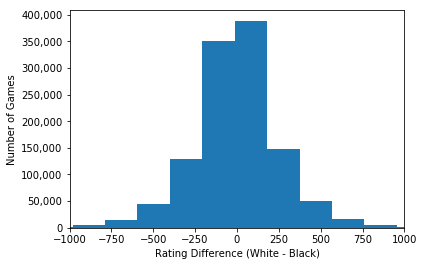
\includegraphics[scale=0.75]{ratinghist}
\end{figure}


%**Notes on data**

%1. Didn't use games between low rated players because low rated players could have %relationships that are bad to learn
%for example, a if white is up a rook, this position should lead to a win 99%+ of the %time, but with bad players this position might lead to a win only 50% of the time %because bad players blunder a lot
%2. further training = neural net plays against itself and one of the player's make a %mistake occassionally
%3. skill level game = sum of 2 players and use this as a weight, rating diff between %players
%4. not super predictable playing style from comp
% Methodology
%	Generally two forms of chess - speed chess and standard chess
%	speed chess more about memorized lines and quickly evaluating new positions
%	standard chess gives player time to think and really consider his move
%   adding a neural net to chess program like standard chess
%	function more complex than std eval funcs and take longer to execute
%	in quick games say 10 secs or less, search is paramount
%	90th percentile for half moves => time for each move
%   use 10 minute time control so that computer has time to think, i.e.
%   adding neural net is like making program more intelligent, without comprising search
%   inevitably # of half moves searched will decrease but hopefully accuracy of eval inc
%   search happen so quickly that full game tree can be explored, then eval = 1 or 0
%   modify TSCP from chessprogramming, run code and profile it, record # of moves per second, # of main eval calls
% modify code and profile it, record # of half moves per second, # of main eval calls, time for eval call
% main eval metric = # of 10 minute time control games won by modified code vs original code and 1 min (or whatever blitz chess is for comp)
% test various feedforward, rnn and cnn neural networks and features
%Data = FICS website, only master level and above games and why
%basic info about the dataset
%# Notes for Report

%1. Vector encoding of board positions
%2. Storage saving from using compressed sparse row matrices
%3. Estimate of time to read 2007 data based on first 1000 games
%4. Parallel processing of the data
%5. graphs - % of white wins, black wins and draws
%6. scatter plot rating diff and white win %
%7. num og games, ave moves per game
%8. randomly check 10 board positions and compare with printed board,
%- max # of 1s for all the boards, ave and min
%- sum of moves = num of rows in sparse matrix
%9. reading first 10,000 games, serial vs parallel



\subsection{Board Encoding}
Since a chess board has 64 squares, and there are 12 different types of pieces, we encoded each board position as a 768-length binary vector. We enumerated the colors, types of pieces, files and ranks as follows:

\begin{description}
	\item[Color:] white (w) = 0, black (b) = 1
	\item[Piece Type:] Pawn (P) = 0, Knight (N) = 1, Bishop (B) = 2, Rook (R) = 3, Queen (Q) = 4, King (K) = 5
	\item[File:] a-file = 0 , b-file = 1, \dots, h-file = 7
	\item[Rank:] 1-file = 0, 2-file = 1, \dots, 8-file = 7.
\end{description}

We then defined the index function $f$ as $f(Color, PieceType, File, Rank) = Color \cdot 384 + PieceType \cdot 64 + File \cdot 8 + Rank$. To encode a board position, we first set all of the elements of the vector to zero, and then for each piece on the board, we set the element at the index given by $f$ to $1$. Thus, a vector could have at most $64$ elements be $1$. To illustrate our encoding of a board position, let $v$ be the encoded vector and consider the position below in Figure \ref{f2}.
\begin{figure}[h!]
	\centering
	\caption{Example Board Position} \label{f2}
	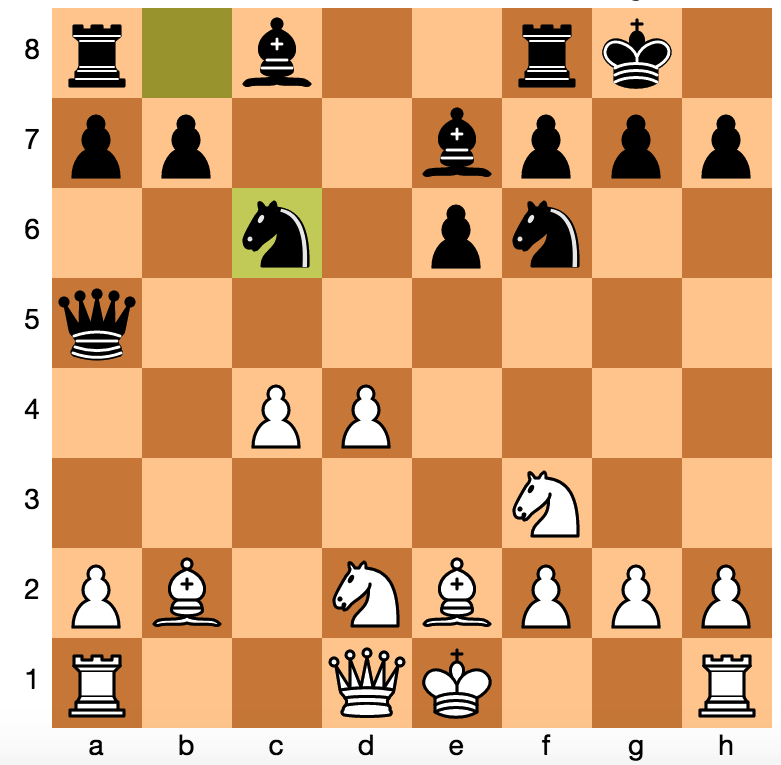
\includegraphics[scale=0.4]{board1}
\end{figure}
For this position, we set $v_i = 1$ for $i =$ 8, 13, 14, 15, 26, 27, 75, 85, 137, 140, 192, 199, 259, 324, 428, 432, 433, 437, 438, 439, 490, 493, 564, 570, 632, 637, 672 and 766 and $v_i = 0$ for the remaining indices.

\subsection{Neural Network Architecture}

We used a feed-forward neural network with three layers as our board evaluation function. The input layer consisted of 768 nodes. The hidden layer consisted of 32,000 nodes with a rectified linear activation function, and the output layer consisted of 3 nodes with a softmax function in order to compute the probability a board position resulted in a win, draw or loss for white. We used one-hot vectors to encode the outcome of a game. For our loss function, we used cross-entropy and decided against using any regularization because of the large volume of data. Since training a neural network can take several hours to days depending on the amount of the data and the size of the neural network, we used a two step process to determine the number of hidden nodes. We first used a sample of the data to determine a reasonable ratio for the number of board positions to the number of hidden nodes. We then multiplied this ratio by the number of board positions in the full data set to arrive at the number of hidden nodes to use. The sample data consisted of 294,428 board positions of which 261,013 were unique. We split the sample data into a training set and a testing set, and for a range of hidden nodes, we trained a neural network and calculated the training loss and testing loss. By comparing the training loss to the testing loss, we determined that 100 nodes was a reasonable amount. From this, we rounded $(96,239,309 / 294,428 \cdot 100)$ to the nearest thousand to attain 32,000 as a reasonable number of hidden nodes. Finally, we trained the neural network on the full data set.

\begin{figure}[h!]
	\centering
	\caption{Learning Curve} \label{f3}
	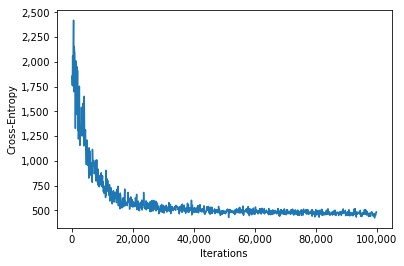
\includegraphics[scale=0.8]{learning}
\end{figure}

\section{Results and Discussion}
% 3 different chesss positions and scores from nn and traditional func

\section{Conclusion}

\bibliographystyle{plain}
\bibliography{bib.bib} 


\end{document}
